\documentclass{article}
\usepackage{graphicx}
\usepackage{float}
\usepackage{tikz}
\usetikzlibrary{trees}

\title{Filesystem Data Structures Report}
\author{Muhammad Arsalan Hussain mh07607}
\date{\today}

\begin{document}

\maketitle

\section{Introduction}

This report describes the data structure used in a filesystem implementation. The data structure comprises a tree/linked-list hybrid to organize files and directories. We will explain the structure and algorithms for traversal and size propagation.

\section{Data Structures}

The filesystem uses several data structures to manage files and directories. These structures include:

\subsection{Directory Entry Structure}

The \texttt{dirent} structure represents an entry in a directory. It includes fields such as:
\begin{itemize}
    \item \texttt{name}: The name of the file or directory.
    \item \texttt{namelen}: The length of the entry name.
    \item \texttt{inode}: The index of the associated inode.
\end{itemize}

\subsection{Node Structure}

The \texttt{Node} structure represents a node in the filesystem's tree/linked-list structure. It includes fields for a \texttt{dirent} entry, as well as pointers to child, sibling, and parent nodes.

\section{Traversal Algorithm}

The traversal algorithm is used to navigate the filesystem tree structure. The primary function, \texttt{traverseUntilParent}, takes a path and traverses the tree until it reaches the parent directory of the target file or directory. The algorithm works as follows:
\begin{enumerate}
    \item Start at the root node.
    \item Iterate through each component of the path, moving to the corresponding child node.
    \item Check if the current node exists and has the correct name. If not, return an error.
    \item Ensure that the target node is a directory (not a file) if needed.
    \item If successful, return 0; otherwise, return -1.
\end{enumerate}

\section{Size Propagation Algorithm}

The size propagation algorithm updates the sizes of parent directories when files or subdirectories are added or removed. It ensures that directory sizes reflect the total size of their contents.

The algorithm works as follows:
\begin{enumerate}
    \item When creating or deleting a file or directory, calculate its size change.
    \item Traverse the tree upward to the root, updating the size of each parent directory by adding or subtracting the size change.
    \item Repeat this process until the root is reached.
\end{enumerate}

\section{Traversal Example}

\begin{figure}[H]
    \centering
    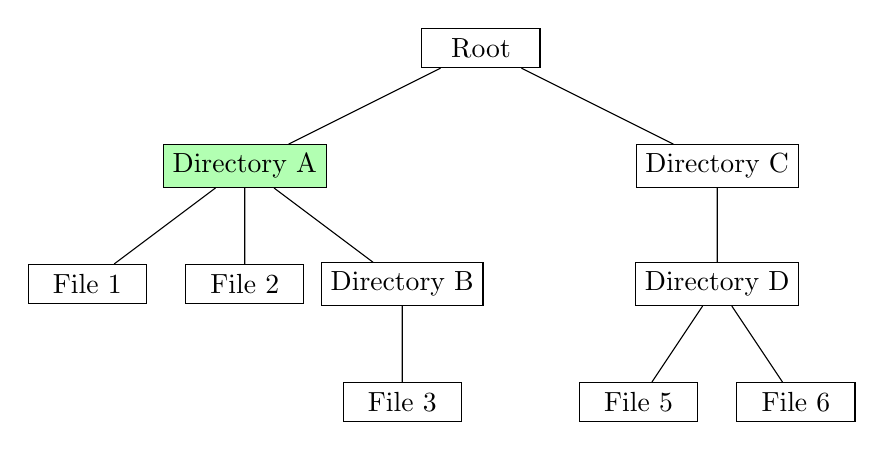
\begin{tikzpicture}[
        level 1/.style={sibling distance=6cm},
        level 2/.style={sibling distance=2cm},
        level 3/.style={sibling distance=2cm},
        every node/.style={draw, rectangle, minimum width=1.5cm, minimum height=0.5cm}
    ]
    \node {Root}
        child {
            node [fill=green!30] {Directory A}
            child {
                node {File 1}
            }
            child {
                node {File 2}
            }
            child {
                node {Directory B}
                child {
                    node {File 3}
                }
            }
        }
        child {
            node {Directory C}
            % child {
            %     node {File 4}
            % }
            child {
                node {Directory D}
                child {
                    node {File 5}
                }
                child {
                    node {File 6}
                }
            }
        };
    \end{tikzpicture}
    \caption{Traversal Example}
\end{figure}

\begin{enumerate}
    \item Start at the \textbf{Root} node.
    \item Move to the first child, \textbf{Directory A}.
\end{enumerate}

\begin{figure}[H]
    \centering
    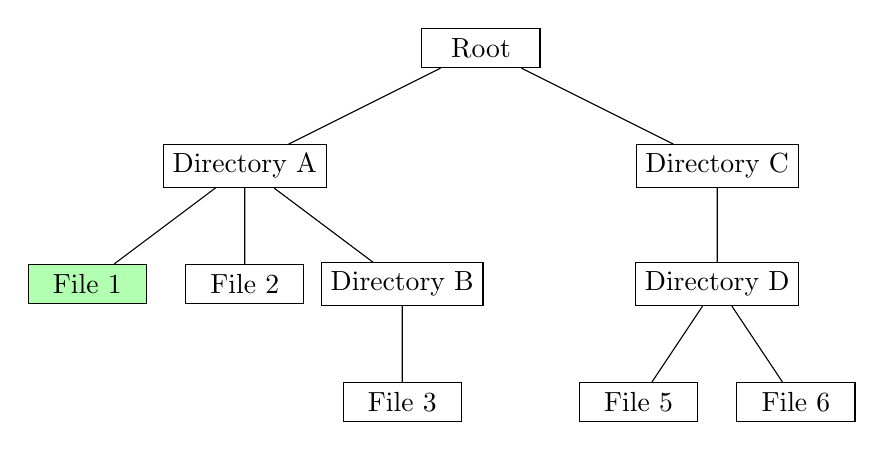
\begin{tikzpicture}[
        level 1/.style={sibling distance=6cm},
        level 2/.style={sibling distance=2cm},
        level 3/.style={sibling distance=2cm},
        every node/.style={draw, rectangle, minimum width=1.5cm, minimum height=0.5cm}
    ]
    \node {Root}
        child {
            node {Directory A}
            child {
                node [fill=green!30] {File 1}
            }
            child {
                node {File 2}
            }
            child {
                node {Directory B}
                child {
                    node {File 3}
                }
            }
        }
        child {
            node {Directory C}
            % child {
            %     node {File 4}
            % }
            child {
                node {Directory D}
                child {
                    node {File 5}
                }
                child {
                    node {File 6}
                }
            }
        };
    \end{tikzpicture}
    \caption{Traversal Example}
\end{figure}


\begin{enumerate}
    \item Inside \textbf{Directory A}, locate \textbf{File 1}.
    \item File not found. Move to the next sibling, \textbf{File 2}.
\end{enumerate}

\begin{figure}[H]
    \centering
    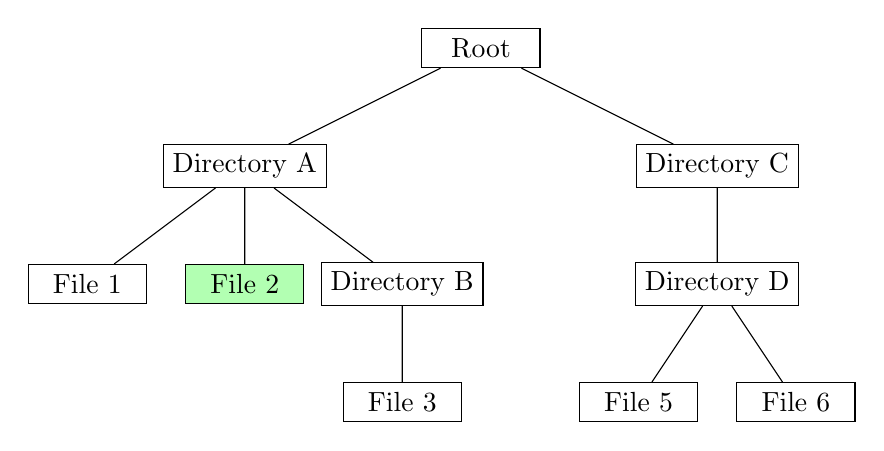
\begin{tikzpicture}[
        level 1/.style={sibling distance=6cm},
        level 2/.style={sibling distance=2cm},
        level 3/.style={sibling distance=2cm},
        every node/.style={draw, rectangle, minimum width=1.5cm, minimum height=0.5cm}
    ]
    \node {Root}
        child {
            node {Directory A}
            child {
                node {File 1}
            }
            child {
                node [fill=green!30] {File 2}
            }
            child {
                node {Directory B}
                child {
                    node {File 3}
                }
            }
        }
        child {
            node {Directory C}
            % child {
            %     node {File 4}
            % }
            child {
                node {Directory D}
                child {
                    node {File 5}
                }
                child {
                    node {File 6}
                }
            }
        };
    \end{tikzpicture}
    \caption{Traversal: Found "File 2"}
\end{figure}

\begin{enumerate}
    \setcounter{enumi}{4}
    \item File found! "File 2" has been located within \textbf{Directory A}.
\end{enumerate}

\section{File and Directory Operations}

The report briefly describes file and directory operations, such as creating and deleting files and directories. These operations involve manipulating the tree structure, updating inodes and block pointers, and propagating size changes.

\section{Conclusion}

In conclusion, the filesystem implementation utilizes a tree/linked-list hybrid data structure to organize files and directories. Traversal and size propagation algorithms ensure efficient navigation and accurate size information.

\end{document}
